% The (r,theta) unit square mapped by c to a polar disk cell.
% Source: book/tex/diffgeo/stokes.tex (§ Cells).
\documentclass[border=2mm]{standalone}
\usepackage{tikz}\usetikzlibrary{arrows.meta}\usepackage{amssymb}
\begin{document}
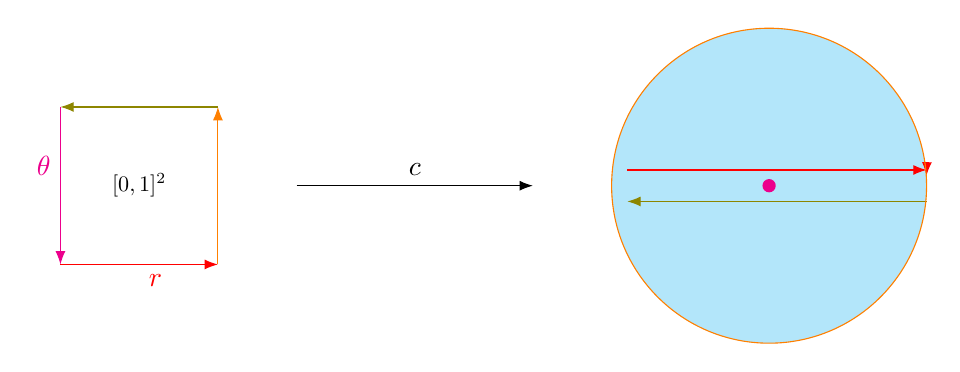
\begin{tikzpicture}[>={Latex}]
  \draw[red,->] (0,0)--(2,0) node[midway,below right]{$r$};
  \draw[orange,->] (2,0)--(2,2); \draw[olive,->] (2,2)--(0,2);
  \draw[magenta,->] (0,2)--(0,0) node[midway,above left]{$\theta$};
  \node at (1,1) {\scalebox{0.8}{$[0,1]^2$}};
  \draw[->] (3,1)--(6,1) node[midway,above]{$c$};
  \fill[cyan!30] (9,1) circle (2);
  \draw[red,->] (9,1.2)++(0:2) arc[start angle=0,end angle=-2,radius=2] ;
  \draw[red,->] (7.2,1.2)--(11,1.2);
  \draw[olive,->] (11,0.8)--(7.2,0.8);
  \draw[orange,->] (9,1) circle (2);
  \fill[magenta] (9,1) circle (2.4pt);
\end{tikzpicture}
\end{document}
